\documentclass[12pt,a4paper]{article}

\usepackage[utf8]{inputenc}
\usepackage[T1]{fontenc}
\usepackage[french]{babel}

\usepackage{amsmath, amssymb}

\usepackage{graphicx}
\usepackage{caption}

\usepackage{siunitx} % Pour les unités

\usepackage{geometry}
\geometry{top=2cm, bottom=2.5cm, left=3cm, right=3cm}
\setlength{\parindent}{0pt}

\usepackage[sfdefault]{roboto}

\usepackage{enumitem}

\usepackage{hyperref}

\usepackage{xcolor}

\usepackage{multicol}
\setlength{\columnseprule}{1pt}
\def\columnseprulecolor{\color{gray}}


\usepackage{import}
\usepackage{xifthen}
\usepackage{pdfpages}
\usepackage{transparent}
\usepackage{float}


\usepackage{multicol}


\newcommand{\incfig}[1]{%
	\def\svgwidth{\columnwidth}
	\import{./figures/}{#1.pdf_tex}
}



\title{Ouvrages spéciaux}
\author{}
\date{\today}

\begin{document}
	
	\maketitle
	
	\tableofcontents
	
	\newpage
	
	\part{Chapitre 1 : Conception et dimensionemment des ponts}
	
	
	\section{Éléments d'un pont}
	
	
	\begin{figure}[H]
		\centering
		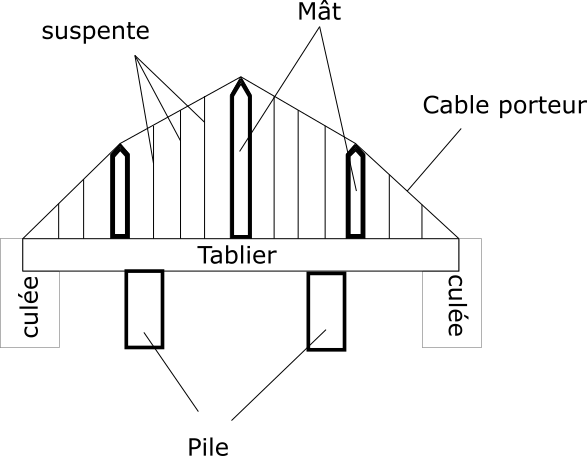
\includegraphics[width=0.7\linewidth]{figures/elements-dun-pont}
		\caption{Éléments d'un pont}
		\label{fig:elements-dun-pont}
	\end{figure}
	
	
	\begin{multicols}{2}
		
		\begin{figure}[H]
			\centering
			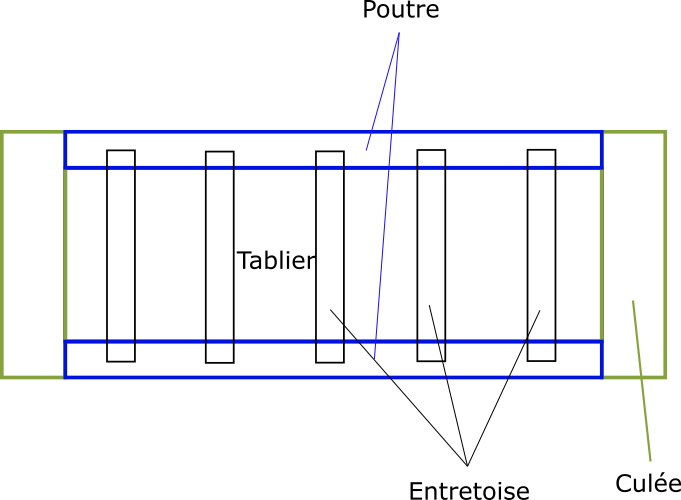
\includegraphics[width=1\linewidth]{figures/elements-du-tablier}
			\caption{Éléments du tablier}
			\label{fig:elements-du-tablier}
		\end{figure}
		
		\columnbreak
		
		\begin{figure}[H]
			\centering
			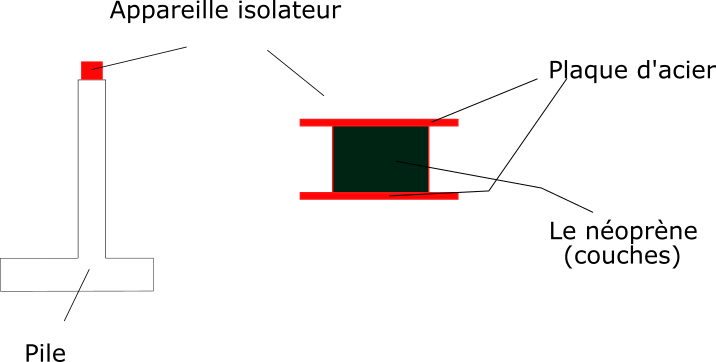
\includegraphics[width=1\linewidth]{figures/elements-pile}
			\caption{Élément de la pile}
			\label{fig:elements-pile}
		\end{figure}
		
	\end{multicols}
	
	\section{Classification des ponts}
	
	\begin{itemize}
		\item Detérmination de la voie portée (tablier).
		\item L'usage : Pont-route, point-rail, pont-aquaduc(avec canalisation d'eau,etc).
		\item Matériaux employé pour les éléments porteur.
	\end{itemize}
	
	
	
	
	
	
	
	
	
	
	
	
	
	
	
	
	
	
	
	
	
	
	
	
	
	
	
	
	
	
	
	
	
	
\end{document}